%% It is just an empty TeX file.
%% Write your code here.

\documentclass[11pt]{article}
\usepackage[margin=1in]{geometry}
\usepackage{amsfonts, amsmath, amssymb}
\usepackage[none]{hyphenat}
\usepackage{fancyhdr}
\usepackage{graphicx}

\pagestyle{fancy}
\fancyhead{}
\fancyfoot{}
\fancyhead[L]{\slshape \MakeUppercase[Place Title Here]}

\DeclareMathOperator*{\argminA}{arg\,min} % Jan Hlavacek
\DeclareMathOperator*{\argminB}{argmin}   % Jan Hlavacek

\begin{document}

\section{Introdution}
As we know, people mostly get information and knowledge from news and articles. In this era, people are also used to using internet doing everything. So it’s no doubt that online news and articles are playing a very important role in our daily life. We can get any news we want through internet quickly. And also, it’s much easier to figure out which online news or articles we like through many internet ways, such like shares, likes and comments. 

As we can imagine, popular news can make the authors become famous, also it can help the social media company attract more people. So they can make more profits. So if an author can know what can make news or articles become popular, or one company can predict whether news or articles will be popular before them are published, they will definitely try their best to get the information. 

So this project aims to find an method to predict how popular an online article can be before it is published by using several statistic characteristics summarized from it. We use the dataset from UCI Machine Learning Repository. In this dataset, it uses the number of shares for an online article to measure how popular it is. It contains 39644 observations with 60 variables, including 2 variables that are not used in orginal work for the dataset, but we will also one of them to build the model. So we will use 59 variables.

The input of algorithm is several features of Mashable articles: Words(e.g. number of words in the title), Links(e.g. number of Mashable article links), Digital Media(e.g. number of images), Time(e.g. day of the week), Keywords(e.g. number of keywords) and Natural Language Processing(e.g. closeness to top 5 LDA topics).

We will predict the popularity in two perspectives. Firstly, we can use regression models(e.g. regression, GAM, Lasso) to predict the number of shares. Secondly, we make articles into 3 levels (unpopular, normal, popular) and then use classification algorithm(e.g. SVM, Random Forest, KNN) to find the articles level.  

\section{Method}
\subsection{Linear models}  
Linear models has been developed in age before computer came out, but we still study and use them a lot. If we have an input vector $X^T=(X_1,X_2,...,X_p)$, and want to predict a output Y. The linear regression model has the form $$Y=\beta_0+\sum_{j=1}^{p} X_j\beta_j$$
The linear model has one of assumptions. The regression function E(Y$\mid$X) is linear or it's reasonable to approximate it into linear model. In this formula, $\beta_j$s are unknown parameters, and variables $X_j$ can be in different sources.  
Also, there are seveal assumptions made for this model. We always assume that E(Y$\mid$X)=f(X) is a linear function of X and the error follows $\epsilon \sim \mathcal N(0, \sigma^2I)$ and $\epsilon$ uncorrelated with X and X is full rank which implies that X^T $\text{ is nonsingular and positive definite.}$

\subsection{Least Absolute Selection and Shrinkage Operator(lasso)}  
Lasso is another method for estimation in linear models. It solves the problem $$\min_{\beta} \sum_{i=1}^{n} (y_i-\sum_{j=1}^{p} x_{ij}\beta_{ij})^2 \text{, subject to } \sum_{j=1}^{p} \lvert \beta_j \rvert \leq t$$
Where t $\geq$ 0 is a parameter given by users. It controls the amount of shrinkage that is applied to the estimates. For the full least squares estimates $\hat{\beta}^0_j$, we can get $t_0=\sum_{j=1}^{p} \lvert \hat{\beta}^0_j \rvert$. $\forall t \leq t_0$ some $\beta_j$ will go to 0. We can also write as $$\hat\beta^{lasso}=\argminB_{\beta \in \mathbb{R}^p} \lVert y-X\beta\rVert^2_2+\lambda\lVert \beta \rVert_1$$
Where $\lambda=0$ gives ordinary least squares, $\lambda\to\infty$ gives $\hat\beta^{lasso}\to0$. 

\subsection{Generalized Additive Models(GAM)}  
Linear models are good, but as the effects are often not linear in the real world, linear models often fail. We can use some more flexible statistical methods that can show nonlinear effects. We call these methods "generalized additive models". If we have an input vector $X^T=(X_1,X_2,...,X_p)$, and want to predict a output Y. The additive model has the form $$Y=\alpha+\sum_{j=1}^{p} f_j(X_j)+\epsilon$$
Where the mean of error term $\epsilon$ is 0. As each $f_j$ is an unspecified smooth nonparametric function. The approach is using an algorithm for simultaneously estimating all functions instead of expanding each function then fitted by simple least squares. Given observation $x_i$, $y_i$, the criterion is like: $$\sum_{i=1}^{N} (y_i-\alpha-\sum_{j=1}^{p}f_j(X_{ij}))^2+\sum_{j=1}^{p} \lambda_jf_j(X_{ij})$$

\subsection{Support Vector Machines(SVM)}  
Besides the regression models, we can also classification algorithm to describe the result. Support Vector Machines are technique for constructing an optimal separating hyperplane between two classes. We can define SVM model as:$$\text{max }L(\alpha)=\sum_{i=1}^{n} \alpha_i - \frac{1}{2}\sum_{i=1}^{n}\sum_{i'=1}^{n}\alpha_i \alpha_i' y_i y_{i'} K(x_i,x_{i'})$$
    \begin{align}
        &s.t.  &0=\sum_{i=1}^{n} \alpha_iy_i \nonumber \\
        &      &0 \leq \alpha_i \leq C \nonumber
    \end{align}
Where the $K(x_i,x_{i'})$ is the kernel function. For this dateset, I try to use linear kernel and radial kernel.
    \begin{align}
        &\text{linear kernel}  &K(x_i,x_{i'})=<x_i,x_{i'}> \nonumber \\
        &\text{radial kernel}  &K(x_i,x_{i'})=exp(-\gamma \lVert x_i-x_{i'} \rVert^2) \nonumber
    \end{align}
For a multiclass classification, if we have K classes total, we can build K(K-1)/2 decision boundaries to decide one point should be put in which class.

\subsection{Random Forest} 
Random Forest is imporved from bagging. In bagging, we build a number of decision trees on bootstrapped training samples from the orginal dataset, and get the final prediction by using the most frequent class of all trees. But for growing the tree from the bootstrapped data, we select m variables at random from the p variables, instead of using all p variables to pick the best variables/split-point. With this idea, we can reduce the variance compared with bagging, by reducing the correlation between the trees.

\subsection{K-Nearest Neighbors(KNN)} 
This idea can be used both in regression and classification. The main thought is we try to estimate the result of x using the k points which are nearest to the x. For this dataset, we use Euclidean distance, and only use the most frequent class from k point to estimate the class of x.

\section{Data Analysis}
\subsection{Diagnostics}
For linear model: \\
    We don't choose a subset of feature to run the regression, as the dataset is not such large. From the fitted vs residual plot we can find that it goes well at the beginning, but as fitted value getting bigger the residuals become not so well. But we can still think the residuals are equally spreaded around a horizontal line without distinct patterns, so there is no non-linear relationships.   \\
    
    \begin{figure}[h]
        \centering
        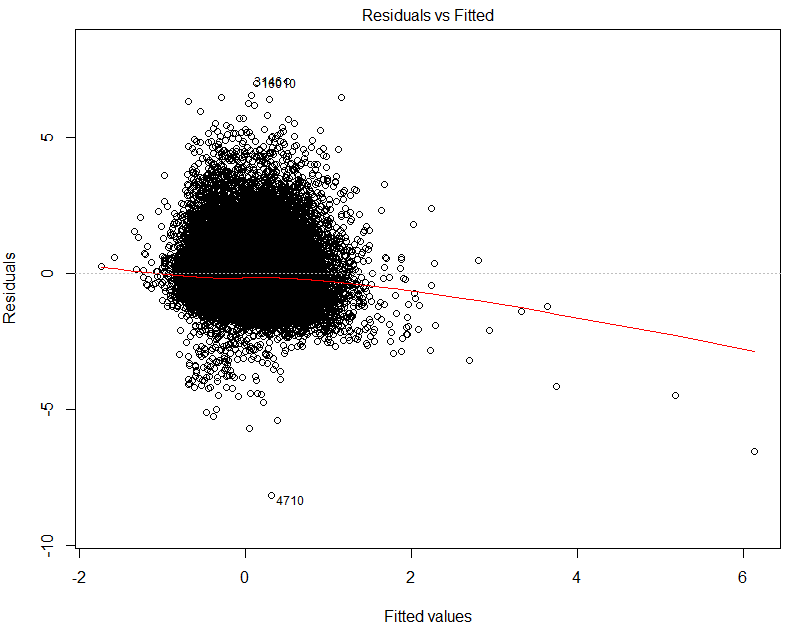
\includegraphics[width=0.7\linewidth]{linear_fvsr.png}
        \caption{Linear Regression Plot: Fitted vs Residuals}
    \end{figure}  
    
    As we look QQ plot, it shows that the residuals are not normally distributed so well. So we should have a concern about the residuals distribuion.\\
    
    \begin{figure}[h]
        \centering
        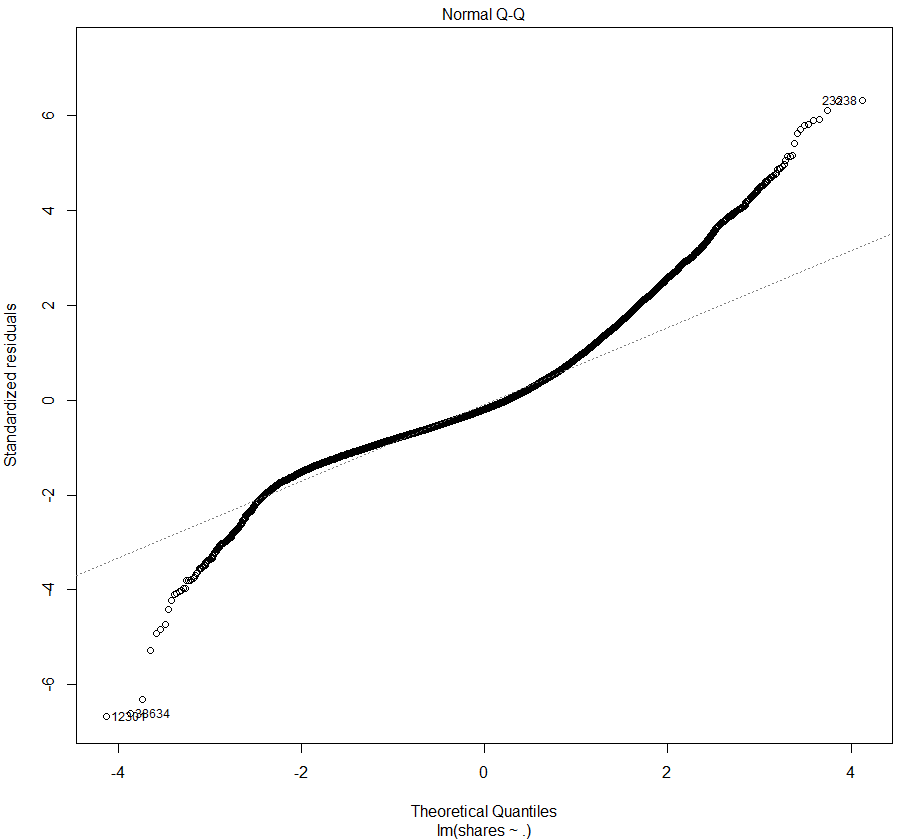
\includegraphics[width=0.7\linewidth]{linear_qq.png}
        \caption{Linear Regression Plot: QQ plot}
    \end{figure}    
    
    From the Scale-location plot, we can see the red line is continually going up, which suggests that the assumptions of equal variance of the residuals may not be true.  \\
    
    \begin{figure}[h]
        \centering
        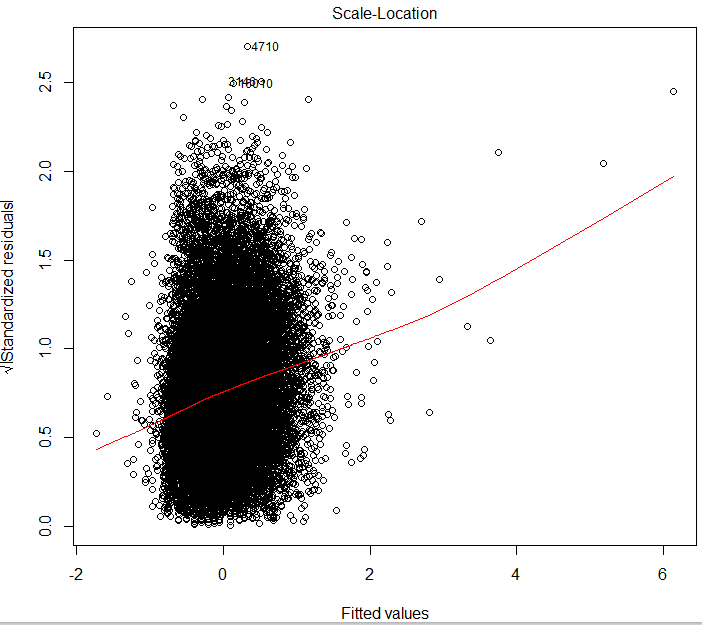
\includegraphics[width=0.7\linewidth]{linear_sl.png}
        \caption{Linear Regression Plot: Scale-location}
    \end{figure}
    
    For all variables, I calculate the vif for each of the variable, and some of their vif value are larger than 10, which shows the collinearity is significant in these variables. And we maybe can think about remove them. \\ 
    
For GAM: From the method part, we know that $f_j(x_j)$ converges from $E \left[Y-\sum_{k \neq j}f_k(x_k)\mid{x_j} \right]$. We use gam model in R to fit the whole dataset, and according to model we get, we know that the number of local scoring iterations used to compute the estimates is only 9, which shows that this method converges pretty fast.
\subsection{Result}
\subsubsection{Regression}
To compare each method result, we decide to separate the whole dataset into training and testing part. We use 70\% of the data to train each model, and then use the rest one to test the error. For regression model, we compare the MSE among linear regression, lasso and GAM. Before training the model, we look the distribution of the number of shares, it seems like the log of number of shares follows normal distribution. So we normalize the log of number of shares and other variables by their mean and variance.\\

    \begin{figure}[h]
        \centering
        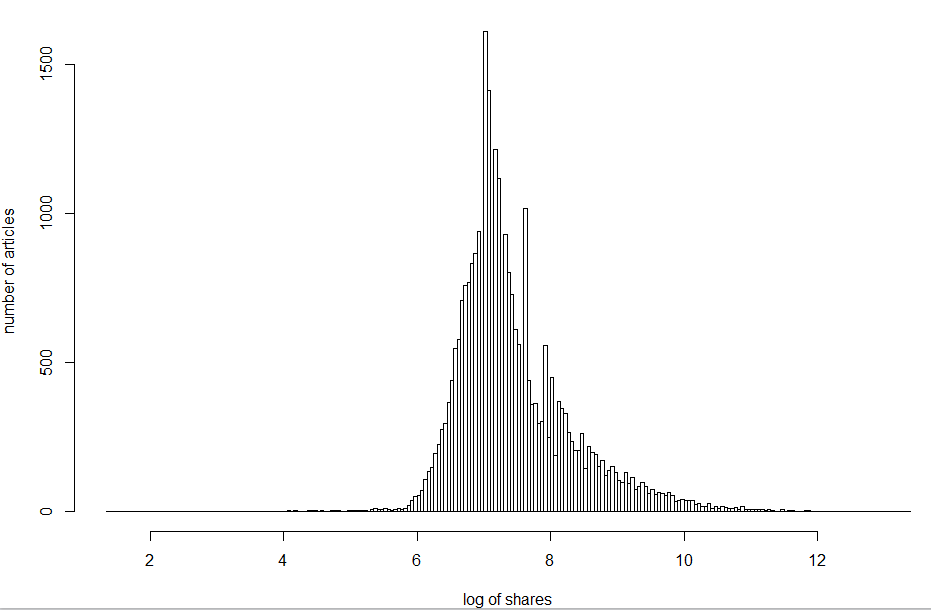
\includegraphics[width=0.7\linewidth]{logy.png}
        \caption{Histogram of log(shares) in training dataset}
    \end{figure}

For the linear regression model, we use all variables including timedelta which is not included in the orginal parper for this dataset. We gets MSE of 1.268389. \\

The lasso gives the MSE of 1.269729. We use cross-validation method first to decide the lambda, after the cross-validation, we use the lambda that gives the minimum MSE to train the model, then get the test MSE. As we can see from Figure \ref{fig:lasso}, the left vertical dash line is the lambda that gives minimum MSE, and the right one is the largest value of lambda such that error is within one standard error of minimum. The number above Figure \ref{fig:lasso} is the number of features chosen by lasso. \\

    \begin{figure}[h]
        \centering
        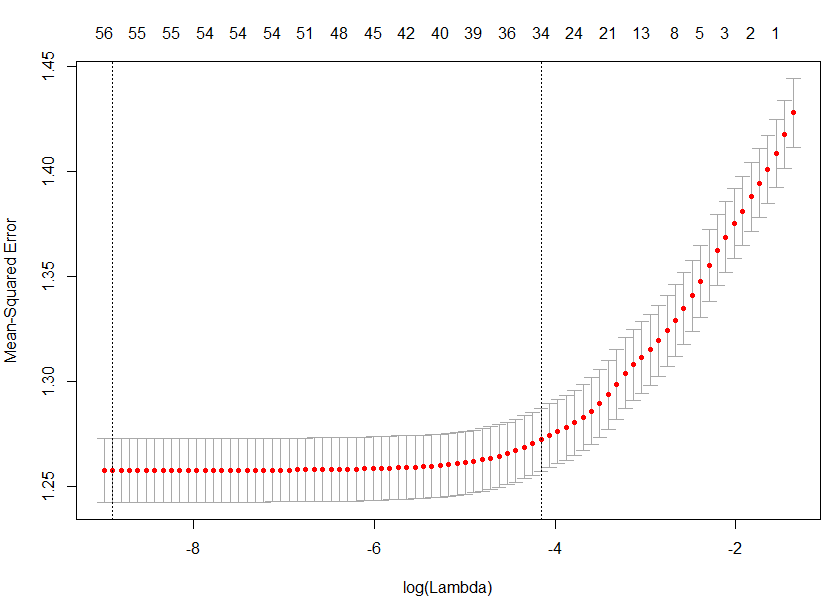
\includegraphics[width=0.7\linewidth]{lasso_plot.png}
        \caption{lasso}
        \label{fig:lasso}
    \end{figure}
    
For GAM, we try to apply smoothing splines to numeric variables. Firstly, we tried the smoothing splines with degree of freedom from 1 to 8. Using cross-validation method, we get the best model is when the degree of freedom is 6 (See from Figure \ref{fig:gam}). After choose the degree of freedom, we get the testing MSE 1.225438. \\ 

    \begin{figure}[h]
        \centering
        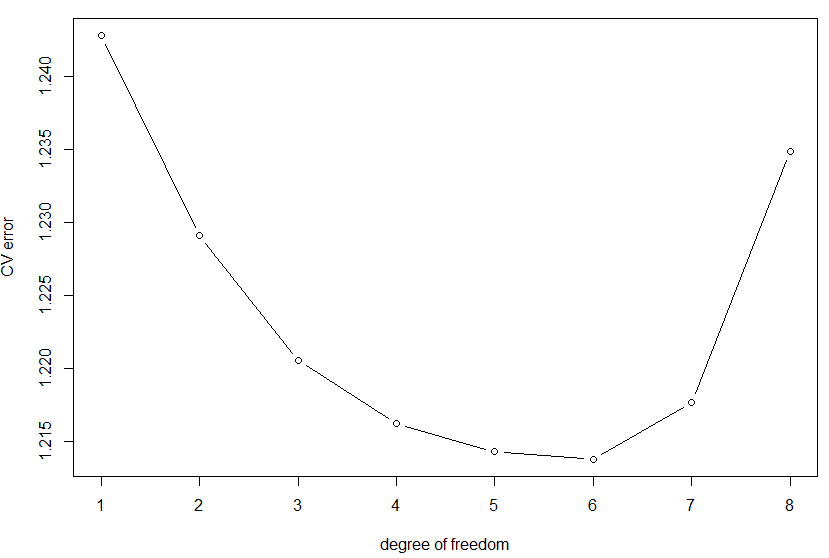
\includegraphics[width=0.7\linewidth]{gam_plot.png}
        \caption{GAM with smoothing spline with different df}
        \label{fig:gam}
    \end{figure}

    \begin{table}[h]
        \centering
        \caption{MSE for Regression}
        \begin{tabular}{ l | r }
            \hline\hline
            Regression model & Testing MSE\\
            \hline
            linear regression & 1.268389 \\
            lasso & 1.269729 \\
            GAM & 1.225438 \\
            \hline\hline
        \end{tabular}
        \label{table:1}
    \end{table}

From the regression models, we can find that the MSEs are not so different from each other. We can't tell which is the best by only looking at the testing MSE. As we think that the exact share number is not a big deal when the number of share is extreme large or extreme small, we can split the response into three categorical level, and give a classifcation prediction.

\subsubsection{classification}
As we know, most of the articles have a very normal number of shares, only a few articles have very large or small number of shares. According to the training dataset, we decide to label the number of shares into three levels (unpopular, normal and popluar) shown in Table \ref{table:Popularity}. \\

    \begin{table}[h]
        \centering
        \caption{Popularity categories}
        \begin{tabular}{ l | r }
            \hline\hline
            The interval of log(shares) & Popularity\\
            \hline
            $\left[$0, 6.6746) & Unpopular \\
            $\left[$6.6746, 8.3894) & Normal \\
            $\left[$8.3894, $\infty$) & Popular \\
            \hline\hline
        \end{tabular}
        \label{table:Popularity}
    \end{table}

    \begin{figure}[h]
        \centering
        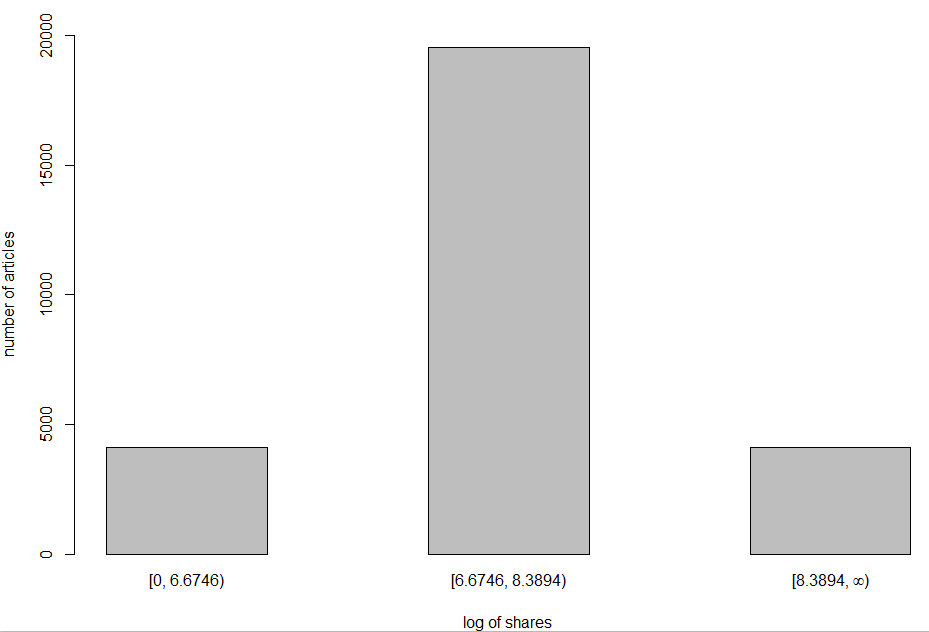
\includegraphics[width=0.7\linewidth]{poplularity.png}
        \caption{Popularity categories}
    \end{figure}

For the one vs one SVM model, we try two different kernel, linear or radial. For the linear kernel, we try C = 0.1, 1, 10, 100, 1000, and use the 10-fold cross-validation method in the training dataset to get the best value for parameter C is . And we also use the radical method and try C = 0.1, 1, 10, 100, 1000 together with $\gamma$ = 0.25, 0.5, 1, 2, 4. Then we still use the 10-fold cross-validation method to get the best C = 0.1 and $\gamma$ = 0.25. So we can get the testing accuracy for best linear is and for best radical is 0.4429.

    \begin{table}[h]
        \centering
        \caption{Confusion Matrix for SVM (radical kernel, C = 0.1, $\gamma$ = 0.25)}
        \begin{tabular}{ c | c | c | c | c }
            \hline\hline
            {} & \multicolumn{4}{c}{Reference} \\
            \hline
            Predition & Unpopular & Normal & Popular & Accuracy\\
            \hline
            Unpopular & 0 & 0 & 0 & 0.NaN\\
            \hline
            Normal & 4871 & 5268 & 1754 & 0.4429\\
            \hline
            Popular & 0 & 0 & 0 & NaN\\
            \hline\hline
        \end{tabular}
        \label{table:knn}
    \end{table}

The random forest gives the accuracy 0.4458085 with the m = 9. We can try the number of variables from 1 to 60, and build 4000 trees. This time we use the out-of-bag (OOB) error estimation instead of cross-validation error as R can give the OOB error directly. The OOB means we can leave only one data from the training dataset, and use other data to fit the random forest model, then use the error from predict the last one. We can find that when m = 9 will give the best accuracy in the training dataset. 

    \begin{figure}[h]
        \centering
        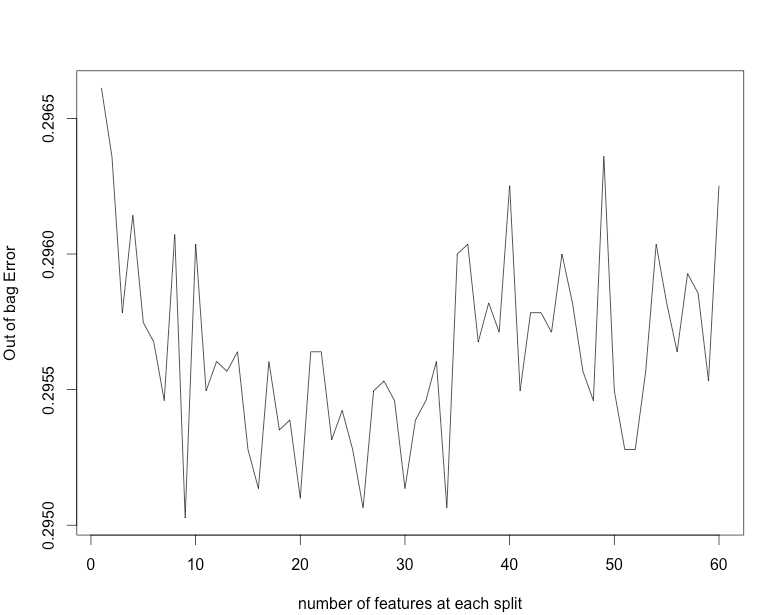
\includegraphics[width=0.7\linewidth]{randomforest_oob.png}
        \caption{Out-of-bag error for different m}
    \end{figure}
    
    \begin{table}[h]
        \centering
        \caption{Confusion Matrix for random forest (m = 9)}
        \begin{tabular}{ c | c | c | c | c }
            \hline\hline
            {} & \multicolumn{4}{c}{Reference} \\
            \hline
            Predition & Unpopular & Normal & Popular & Accuracy\\
            \hline
            Unpopular & 57 & 28 & 1 & 0.662791\\
            \hline
            Normal & 4799 & 5224 & 1732 & 0.44441\\
            \hline
            Popular & 15 & 16 & 21 & 0.403846\\
            \hline\hline
        \end{tabular}
        \label{table:rf}
    \end{table}

The confusion matrix in Table \ref{table:rf} shows that we can predict Unpopular some how well, and Nomarl and Popular can still be predicted correct for the majority.

For KNN, we try k from 1 to 100, which means we wish to find the best number of points in dataset to represent the point we want to predict. We use the cross-validation method, and find out that best number of points is 55. We get the testing accuracy for KNN is 0.4437064.

    \begin{figure}[h]
        \centering
        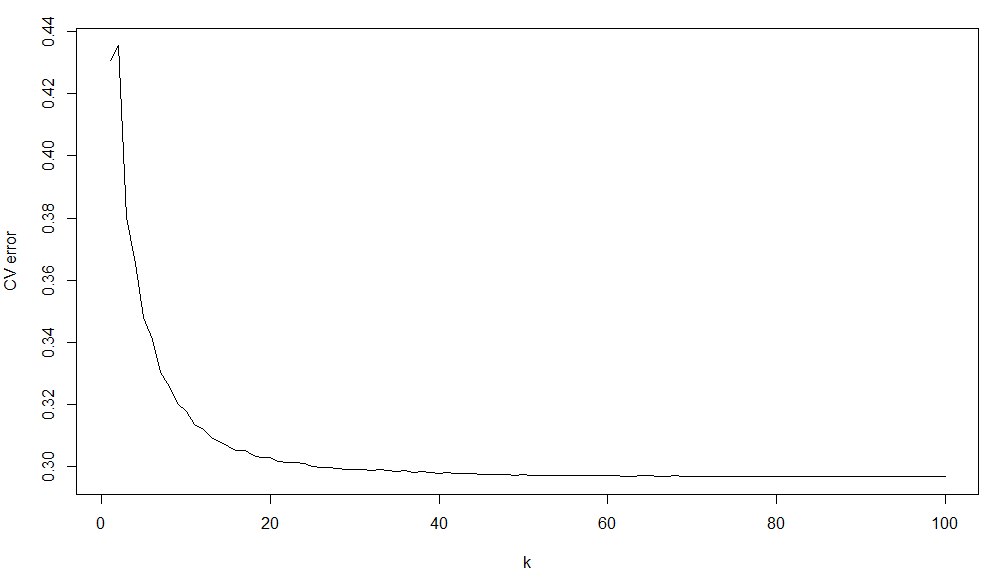
\includegraphics[width=0.7\linewidth]{knn_cv.png}
        \caption{cross-validation error for KNN}
    \end{figure}

    \begin{table}[h]
        \centering
        \caption{Confusion Matrix for KNN (k = 55)}
        \begin{tabular}{ c | c | c | c | c }
            \hline\hline
            {} & \multicolumn{4}{c}{Reference} \\
            \hline
            Predition & Unpopular & Normal & Popular & Accuracy\\
            \hline
            Unpopular & 14 & 5 & 3 & 0.636364\\
            \hline
            Normal & 4857 & 5263 & 1751 & 0.443349\\
            \hline
            Popular & 0 & 0 & 0 & NaN\\
            \hline\hline
        \end{tabular}
        \label{table:knn}
    \end{table}

The confusion matrix in Table \ref{table:knn} shows that we can predict Unpopular some how well, and Nomarl can still be predicted correct for the majority. But knn may be bad for predicting Popular ones, as it even doesn't predict one result popluar.

\section{Conclusion}
In this thesis, we train several regression and classification models to predict the popularity of some online articles before them are published. We use number of shares to judge the popularity of the articles. The data we use is from Mashable news service, providing from UCI Machine Learning Repository.  \\
Over the regression models, the best result was achieved by Generalized Additive Model(GAM) with a testing mean squared error 1.225438 after the normalization for the log of number of shares. As we know, linear regression and lasso are not flexible compared with GAM, which means they are supposed to get a bigger MSE but less variance. As diagnostics we have done, it shows that the variables are more prosible having a non-linear relationship with response. So I think the non-linear model such as GAM could be a good fit for the regression model. \\
As the classification models, the best result goes to random forest with the accuracy 0.4458085. Looking through the confusion matrix, we can find out that only random forest can give a prediction for those articles labeled by Unpopular or Popular.\\
Overall, the work for this thesis gives a new perspective about the reason for influencing the popularity of online articles from a statistics view instead of content or article style.
In the future work, we want to use the method that the orginal thesis gives to get more data from other online articles resources to train a better model, and also try to use more method to give a better prediction.
\section{Appendix}

    \begin{table}[h]
        \centering
        \caption{List of variables}
        \begin{tabular}{ l | l }
            \hline\hline
            Variable names & Type(\#)\\
            \hline
            \multicolumn{2}{c}{Words}\\
            \hline
            Number of words in the title & numeric(1) \\
            Number of words in the content & numeric(1) \\
            Average length of the words in the content & numeric(1) \\
            Rate of unique words in the content & numeric(1) \\
            Rate of non-stop words in the content & numeric(1) \\
            Rate of unique non-stop words in the content & numeric(1) \\
            \hline
            \multicolumn{2}{c}{Links}\\
            \hline
            Number of links & numeric(1) \\
            Number of links to other articles published by Mashable & numeric(1) \\
            Shares of referenced article links in Mashable (min, avg, max) & numeric(3) \\
            \hline
            \multicolumn{2}{c}{Digital Media}\\
            \hline
            Number of images & numeric(1) \\
            Number of videos & numeric(1) \\
            \hline
            \multicolumn{2}{c}{Time}\\
            \hline
            Days between the article publication and the dataset acquisition & numeric(1) \\
            Day of the week (from Monday to Sunday) & binary(7) \\
            The article published on the weekend & binary(1) \\
            \hline
            \multicolumn{2}{c}{Keywords}\\
            \hline
            Number of keywords in the metadata & numeric(1) \\
            Data channel (Lifestyle, Entertainment, Business, Social Media, Tech or World) & binary(6) \\
            Worst keyword shares (min, avg, max) & numeric(3) \\
            Best keyword shares (min, avg, max) & numeric(3) \\
            Average keyword shares (min, avg, max) & numeric(3) \\
            \hline
            \multicolumn{2}{c}{Natural Language Processing}\\
            \hline
            Closeness to top LDA topics from 1 to 5 & numeric(5) \\
            Text subjectivity & numeric(1) \\
            Text sentiment polarity & numeric(1) \\
            Rate of positive words in the content & numeric(1) \\
            Rate of negative words in the content & numeric(1) \\
            Rate of positive words among non-neutral tokens & numeric(1) \\
            Rate of negative words among non-neutral tokens & numeric(1) \\
            Polarity of positive words (min, avg, max) & numeric(3) \\
            Polarity of negative words (min, avg, max) & numeric(3) \\
            Title subjectivity & numeric(1) \\
            Title polarity & numeric(1) \\
            Absolute subjectivity level & numeric(1) \\
            Absolute polarity level & numeric(1) \\
            \hline\hline
        \end{tabular}
        \label{table:1}
    \end{table}

\end{document}